\documentclass[14pt,a4paper]{extarticle}
\usepackage[T2A]{fontenc}
\usepackage[utf8]{inputenc}
\usepackage[english,russian]{babel}
\usepackage{lmodern}
\usepackage{geometry}
\usepackage{array}
\usepackage{tabularx}
\usepackage{longtable}
\usepackage{ltablex}
\usepackage{booktabs}
\usepackage{hyperref}
\usepackage{indentfirst}
\usepackage{microtype}
\usepackage{graphicx}
\usepackage{setspace}
\usepackage{listings}
\usepackage{graphicx}
\usepackage{caption}
\usepackage{float}
\usepackage{tocloft}
\usepackage{titlesec}
\usepackage{newtxtext,newtxmath}

\titleformat{\section}        % форматируем \section
  {\normalfont\bfseries}      % стиль: обычный + жирный
  {\thesection.}              % номер секции с точкой
  {2mm}                       % расстояние между номером и текстом
  {}                           % перед заголовком можно добавить что-то
\titlespacing*{\section}{1.5cm}{*3}{*1}  % {отступ слева}{отступ сверху}{отступ снизу}

\captionsetup{justification=centering}
\renewcommand{\ttdefault}{cmtt}
\keepXColumns
\setlength{\parindent}{3em}
\newgeometry{left=2.5cm,right=2.5cm,top=3cm,bottom=2.5cm}

\renewcommand{\contentsname}{\hspace*{4em}{\smallСодержание}}
\setlength{\cftbeforesecskip}{0.5em}
\renewcommand{\cftsecleader}{\cftdotfill{\cftdotsep}}
\renewcommand{\cftsecaftersnum}{.\hspace{2mm}}

\title{Отчёт по дисциплине "Основы предпринимательства"}
\author{Выполнил студент группы М-РИТ-25-1, Станиславчук Сергей}

\begin{document}

\setstretch{1.5}
\noindent
\begin{minipage}[t]{0.01\textwidth}
    \includegraphics{~/programmer/++Programmer/5_1/LSTU.jpg}
\end{minipage}%
\begin{minipage}[c]{1.1\linewidth}
    \centering
    {\small
    МИНИСТЕРСТВО НАУКИ И ВЫСШЕГО ОБРАЗОВАНИЯ РФ \\[1em]
    ФЕДЕРАЛЬНОЕ ГОСУДАРСТВЕННОЕ БЮДЖЕТНОЕ \\
    ОБРАЗОВАТЕЛЬНОЕ УЧРЕЖДЕНИЕ ВЫСШЕГО ОБРАЗОВАНИЯ \\
    «ЛИПЕЦКИЙ ГОСУДАРСТВЕННЫЙ ТЕХНИЧЕСКИЙ УНИВЕРСИТЕТ»
    }
\end{minipage}%

\vspace{3em}

\noindent
\hspace{1em}%
\begin{minipage}[t]{0.8\textwidth}
\textbf{Институт} \hspace{2em} компьютерных наук \\
\textbf{Кафедра} \hspace{2em} автоматизированных систем управления
\end{minipage}


\vspace{6em}

\begin{center}
\textbf{ПРАКТИЧЕСКАЯ РАБОТА №5} \\
по дисциплине \\ <<Основы предпринимательства>>
\end{center}

\vspace{6em}

\noindent
\begin{tabular*}{\textwidth}{@{\extracolsep{\fill}} l c r }
    Студент М-РИТ-25-1 & \makebox[4cm]{\hrulefill} & Станиславчук С.М. \\[2em]
Руководитель & \\
Канд. юр. наук, доцент & \makebox[4cm]{\hrulefill} & Моисеева И.И. \\
\end{tabular*}

\vfill
\begin{center}
    Липецк, 2025
\end{center}

\thispagestyle{empty}

\newpage
\tableofcontents
\newpage

\section{Задание 1}
\begin{sloppypar}
В 1-м квартале предприятие реализовало 500 изделий по цене 60 руб. за единицу. Во
2-м квартале было реализовано 900 изделий. В третьем квартале было реализовано 700 изд.
Определите доход предприятия от реализации продукции
\end{sloppypar}

Решение.

    $500 * 60 + 900 * 60 + 700 * 60 = 126 000$ - выручка от реализации продукции.
    А доход - это выручка от реализации продукции за вычетом материальных затрат. Данных
    для определения дохода в задаче нет.

    Ответ: 126 000 - выручка, данных для определения дохода недостаточно (оплата труда и прибыль).

\section{Задание 2}
Предприятие, выпускающее бытовую технику, с помощью дорогостоящих
исследований, попыталось усовершенствовать один из выпускаемых товаров. Но никакого
результата эти исследования не принесли, товар остался без изменений. В то же время
надпись «Усовершенствованная новинка» на товаре значительно повысит объем
реализованной продукции.
Какое решение Вы примете: сделаете такую надпись или нет? Почему?

Решение.

С одной стороны это конечно неправильно обманывать своих покупателей, но с другой стороны
если это действительно повысит объем реализованной продукции, даже на первое время, то можно
    попробовать, только если моя фирма на грани банкротсва (в задании указано, что исследования были дорогостоящими).
    Доход с увеличенных продаж даст времени на обдумывание нового плана восстановления репутации, потому что рано
    или поздно ложь выяснится и к фирме уже не будет такого доверия как раньше, и продажи сильно упадут.
    Если же фирме не грозят финансовые проблемы и вложенные в исследования деньги некритично повлияли на изменение
    общего капитала фирмы, на такой рискованный поступок я бы не решился.
    Финансы - это легковосстанавливаемый ресурс, а вот репутацию вернуть очень сложно.

    Если рассматривать первый вариант, то ошибка уже совершена - деньги уже были потрачены на безрезультатные
    исследования. Вопрос в другом, сможет ли фирма также функционировать без изменения в маркетинге как и до
    исследований. Если нет, и прогнозы прибыли фирмы неутешительные (доход 0 или отрицательный), в таком
    случае возможно и стоит рискнуть своей репутацией для выживания на рынке еще какое-то время.
    Второй вариант: оплата дорогостоящих исследований не сильно скажется на состоянии фирмы, то и
    делать для других (сейчас) и себя (в будущем) "подлянку" не стоит.

Ответ: Зависит от ситуации фирмы, см. решение.

\section{Задание 3}
Кондитерское предприятие «Конти-п» занимается производством скоропортящихся
продуктов со сроком хранения не более трех суток. Руководителю предприятия
предложили продавать производимые продукты в другой области, затрачивая время на их
перевозку и, соответственно, уменьшая срок годности. должен ли принять руководитель
предприятия данное предложение? По чему?

Решение.

Здесь, как и в предыдущей задаче, все зависит от ситуации. Если я правильно понял,
в задании "область" является субъектом федерации (Липецкая, Московская и др.).
Все зависит от времени перевозки товара между областями. Так, например, если
производить транспортировку для соседней области, допустим из Липецкой в Тамбовскую
или Воронежскую, то это скажется на увеличении времени транспортировки некритично
(2-4 часа при сроке хранения в 72 часа). В таком случае руководитель обязан согласиться.

При ситуации, когда транспортивка занимает гораздо больше времени, допустим из
Липецкой области в г. Уфа. В среднем около 20-24 часов. Попрошу заметить, это треть
от общего срока хранения товара. Такая ситуация не будет выгодной не для производителей,
не для покупателей. Потому что может сильно увеличить количество просроченной продукции, которую
попросту не успеют купить. В таком случае руководителю стоит отказаться от предложения.

Например, молоко лебедянь, производимое в Липецкой области, тоже является скоропортящимся
продуктом, на их сайте с логистикой https://lmilk.ru/where-buy/ видно (рис.1), что молоко
поставляется только в соседние области, как раз по той же причине: время транспортирки
занимает не более 8 часов времени в каждую область (самая дальняя область - Тверская, 650км,
8 часов езды).

\begin{figure}[H]
    \label{fig:pic1}
    \centering
    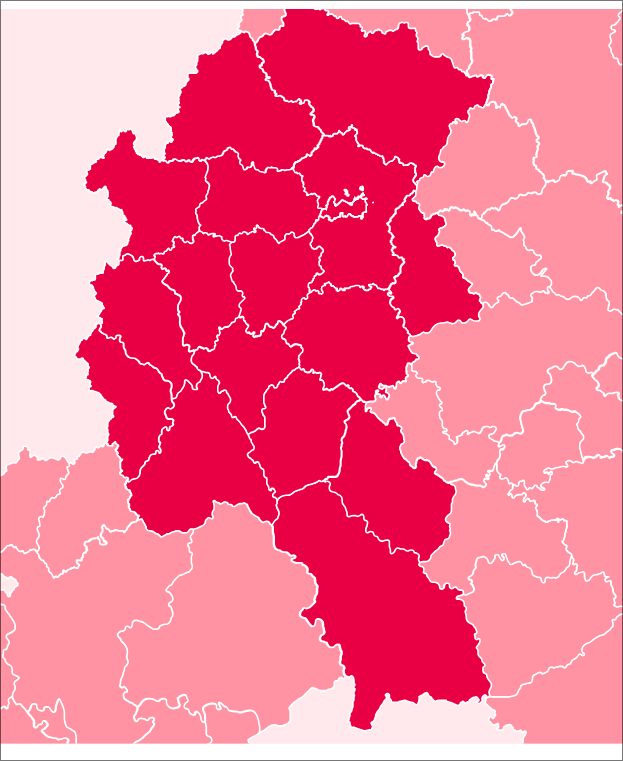
\includegraphics[width=0.78\textwidth]{pic1.png}
    \refstepcounter{figure}
    \caption*{Рисунок \thefigure\ — регионы, в которых продается молоко Лебедянь}
\end{figure}



Ответ: Зависит от времени транспортировки, см. решение.

\section{Задание 4}

Ваше предприятие изо всех сил старается добиться заключения выгодного контракта
на большую сумму продаж с одной компанией. В ходе переговоров Вы узнаете, что
представитель покупателя подыскивает себе более выгодную работу, у вас нет желания
брать его к себе на работу, но если Вы намекнете ему об этой возможности он, скорее
всего, передаст заказ именно вам. Как Вы поступите и почему?

Решение.

Здесь видно встречу двух интересов. Если я помогу найти ему более выгодную
работу, он тоже пойдет мне на встречу, в итоге все получат то, чего хотели. У
представителя покупателя появится возможность устроится на более прибыльную
работу, у меня выгодный контракт.

Остается решить как и куда его можно устроить. В условии сказано, что желания
брать его к себе на работу нет. А обманывать человека точно не собираюсь,
я могу предложить ему поучавствовать в конкурсе на устраивающую его должность,
так будет честно, если он пройдет собеседование и докажет свою компетентность,
у меня и желание появится взять его на работу. Таким образом, я даю ему шанс
устроиться на желаемую им работу, а он мне дает шанс заключить выгодный
контракт.

Ответ: пойду ему на встречу.

\section{Задание 5}

Первоначальная стоимость основных средств 24 000 тыс, руб. Стоимость введенных
в феврале ОСНОВНЫХ средств составила 370 тыс, руб. Стоимость ликвидированных в
сентябре основных средств 280 тыс, руб. Цена единицы продукции 45 руб., а размер
выпуска продукции 700 тыс. шт.
Определите фондоёмкость и фондоотдачу основных средств.

Решение.

Среднегодовая стоимость основных фондов рассчитывается по формуле:
\[
F_{\text{ср}} = F_0 + F_{\text{вв}} \cdot \frac{t_{\text{вв}}}{12}
               - F_{\text{ликв}} \cdot \frac{t_{\text{ликв}}}{12}
\]

\[
F_{\text{ср}} = 24000 + 370 \cdot \frac{11}{12} - 280 \cdot \frac{4}{12}
\]

\[
F_{\text{ср}} = 24000 + 339.17 - 93.33 = 24345.84\ \text{тыс.~руб.}
\]

Объём выпуска в денежном выражении:
\[
Q = 45 \cdot 700000 = 31500000\ \text{руб.} = 31500\ \text{тыс.~руб.}
\]

Фондоотдача:
\[
\text{Фодоот} = \frac{Q}{F_{\text{ср}}}
\]
\[
\text{Фодоот} = \frac{31500}{24345.84} \approx 1.29
\]

Фондоёмкость:
\[
\text{Фондёмк} = \frac{F_{\text{ср}}}{Q}
\]
\[
\text{Фондёмк} = \frac{24345.84}{31500} \approx 0.773
\]

\textbf{Ответ:}

Фондоотдача: \( \approx 1.29 \).
Фондоёмкость: \( \approx 0.77 \).

\section{Задание 6}
Приобретен объект основных средств стоимостью 140 тыс. руб. со сроком полезного
способом уменьшаемого остатка.
использования 4 года.
Определите годовую сумму амортизационных отчислений линейным способом и

Решение.

1) Годовая норма амортизации:
\[
N = \frac{1}{T} = \frac{1}{4} = 0.25 \ (25\%)
\]

Годовая амортизация:
\[
A_{\text{год}} = C \cdot N = 140 \cdot 0.25 = 35\ \text{тыс.~руб.}
\]

2) Увеличенная норма амортизации:
\[
N_{\text{ум}} = 2 \cdot N = 2 \cdot 0.25 = 0.5 \ (50\%)
\]

Амортизация по годам:

\[
A_1 = 140 \cdot 0.5 = 70
\]

\[
A_2 = (140 - 70) \cdot 0.5 = 70 \cdot 0.5 = 35
\]

\[
A_3 = (70 - 35) \cdot 0.5 = 35 \cdot 0.5 = 17.5
\]

\[
A_4 = (35 - 17.5) \cdot 0.5 = 17.5 \cdot 0.5 = 8.75
\]

\textbf{Ответ:}

Линейный способ:
\[
A_{\text{год}} = 35\ \text{тыс.~руб.}
\]

Способ уменьшаемого остатка:
\[
A_1 = 70,\quad A_2 = 35,\quad A_3 = 17.5,\quad A_4 = 8.75\ \text{тыс.~руб.}
\]

\section{Задание 7}
Выпуск продукции за год составил 8 500 ед., себестоимость изделия — 90 руб., цена
изделия на 25 % превышает его себестоимость, среднегодовой остаток оборотных средств
— 45 тыс. руб., длительность производственного цикла изготовления — 4 дня,
коэффициент нарастания затрат в незавершенном производстве — 0,6. Определите
норматив оборотных средств в незавершенном производстве и оборачиваемость
оборотных средств предприятия.

Решение.

Обозначения: год принимаем за $360$ дней (стандарт для подобных задач).
Годовая себестоимость продукции:
\[
S_{\text{год}} = 8500 \cdot 90 = 765000\ \text{руб.}
\]

Средняя дневная себестоимость:
\[
s_{\text{дн}} = \frac{S_{\text{год}}}{360} = \frac{765000}{360} = 2125\ \text{руб./день}
\]

Норматив оборотных средств в незавершённом производстве рассчитывается по формуле
\[
N_{\text{нзп}} = s_{\text{дн}} \cdot t_{\text{ц}} \cdot k_{\text{н}},
\]
где $t_{\text{ц}}$ --- длительность производственного цикла (в днях), $k_{\text{н}}$ --- коэффициент нарастания затрат.

Подставляем:
\[
N_{\text{нзп}} = 2125 \cdot 4 \cdot 0.6 = 2125 \cdot 2.4 = 5100\ \text{руб.}
\]
(что равно $5{,}1\ \text{тыс. руб.}$).

Коэффициент оборачиваемости оборотных средств (в год):
\[
K_{\text{об}} = \frac{S_{\text{год}}}{\text{Среднегодовой остаток оборотных средств}}
= \frac{765000}{45000} = 17\ \text{раз в год}.
\]

Период оборачиваемости (в днях):
\[
T_{\text{об}} = \frac{360}{K_{\text{об}}} = \frac{360}{17} \approx 21.18\ \text{дн.}
\]

\textbf{Ответ:}

Норматив оборотных средств в незавершённом производстве:
\[
N_{\text{нзп}} = 5100\ \text{руб.} \; (5{,}1\ \text{тыс. руб.}).
\]

Оборачиваемость оборотных средств:
\[
K_{\text{об}} = 17\ \text{раз в год}, \qquad T_{\text{об}} \approx 21.18\ \text{дн.}.
\]

\section{Задание 8}
Среднесписочная численность работников предприятия составила 750 чел., в
течение года уволилось по собственному желанию — 17 чел., уволено за нарушение
трудовой дисциплины —8 чел., ушли на пенсию —25 чел.
Определите коэффициенты выбытия и текучести кадров

Решение.

Коэффициент выбытия рассчитывается по формуле:
\[
K_{\text{выб}} = \frac{\text{Все уволенные за год}}{\text{Среднесписочная численность}}.
\]

\[
\text{Все уволенные} = 17 + 8 + 25 = 50\ \text{чел.}
\]

\[
K_{\text{выб}} = \frac{50}{750} = 0.0667 \approx 6.67\%.
\]

Коэффициент текучести кадров включает увольнения по собственному желанию и за нарушение дисциплины:
\[
K_{\text{тек}} = \frac{17 + 8}{750} = \frac{25}{750} = 0.0333 \approx 3.33\%.
\]

\textbf{Ответ:}

Коэффициент выбытия:
\[
K_{\text{выб}} \approx 0.0667 \; (6.67\%).
\]

Коэффициент текучести кадров:
\[
K_{\text{тек}} \approx 0.0333 \; (3.33\%).
\]

\section{Задание 9}
В первом квартале количество выпущенной продукции на предприятии составляет
45 тыс, изделий. Себестоимость одного изделия составляет 52 тыс, руб., а его цена — 61
тыс, руб. Определите рентабельность продукции за отчетный период.

Решение.

Рентабельность продукции обычно вычисляют как отношение прибыли к себестоимости:
\[
R = \frac{P}{C}\times 100\%,
\]
где $P$ --- прибыль на период, $C$ --- себестоимость за период.

Прибыль на единицу:
\[
p = \text{цена} - \text{себестоимость} = 61\,000 - 52\,000 = 9\,000\ \text{руб.}
\]

Общая прибыль за период:
\[
P = p \cdot Q = 9\,000 \cdot 45\,000 = 405\,000\,000\ \text{руб.}
\]

Общая себестоимость за период:
\[
C = 52\,000 \cdot 45\,000 = 2\,340\,000\,000\ \text{руб.}
\]

Рентабельность:
\[
R = \frac{405\,000\,000}{2\,340\,000\,000}\times100\% = \frac{9}{52}\times100\% \approx 17.31\%.
\]

\textbf{Ответ:} $R \approx 17.31\%$.

\section{Задание 10}
Предприятие производит продукцию одного наименования по цене 520 руб. за
единицу, удельные переменные расходы составляют —280 руб., общая величина
постоянных расходов — 750 тыс, руб. В результате роста арендной платы общие
постоянные расходы увеличились на 10 %.
Определите, как изменится величина критического объема

Решение.

Критический (безубыточный) объём определяется формулой:
\[
Q_{\text{кр}}=\frac{F}{p-v}.
\]

Вычислим маржу на единицу:
\[
p-v=520-280=240\ \text{руб./ед.}
\]

Начальный критический объём:
\[
Q_{\text{кр,1}}=\frac{750\,000}{240}=3125\ \text{ед.}
\]

Постоянные расходы после увеличения на $10\%$:
\[
F_2=750\,000\cdot 1.10=825\,000\ \text{руб.}
\]

Новый критический объём:
\[
Q_{\text{кр,2}}=\frac{825\,000}{240}=3437.5\ \text{ед.}
\]

Изменение критического объёма:
\[
\Delta Q = Q_{\text{кр,2}}-Q_{\text{кр,1}} = 3437.5-3125 = 312.5\ \text{ед.}
\]

Обычно объём в штуках округляют вверх, так как дробная часть означает неполную единицу продукции:
\[
Q_{\text{кр,1}}=3125\ \text{ед.},\quad Q_{\text{кр,2}}=3438\ \text{ед.}
\]

\textbf{Ответ (задание 10):}
Критический объём увеличится с $3125$ ед. до примерно $3438$ ед., т.е. рост на $\approx 313$ ед. (точное изменение $312.5$ ед.).

Ответ: 5.88\%

\section{Задание 11}
Объем капитальных вложений по объектам производственного назначения в
развитие одной из подотраслей горнодобывающей промышленности составит 5400000000
руб. Прирост прибыли в рассматриваемом периоде по плану должен составить 930000000
руб.
Определить:
1) общую экономическую эффективность капитальных вложений;
2) отклонения общей эффективности капитальных вложений от норматива;
3) срок окупаемости общих капитальных вложений

Решение.

1) \textit{Общая экономическая эффективность (рентабельность капитальных вложений)} обычно определяется как отношение
прироста прибыли к объёму вложений:
\[
E = \frac{\Delta\Pi}{I}.
\]
Подставляем числа:
\[
E = \frac{930\,000\,000}{5\,400\,000\,000} = 0.172222\ldots \approx 0.17222 = 17.22\%.
\]

2) \textit{Отклонение от норматива.} Обозначим нормативную эффективность через \(E_{\text{норм}}\). Тогда отклонение:
\[
\Delta E = E - E_{\text{норм}}.
\]
Поскольку в условии норматив не задан, численно вычислить \(\Delta E\) невозможно без значения \(E_{\text{норм}}\).
Для иллюстрации приведём отклонения при двух примерных нормативных значениях:

\begin{itemize}
  \item Если \(E_{\text{норм}}=12\%\), то
  \[
  \Delta E = 17.22\% - 12\% = +5.22\ \text{п. п.}
  \]
  \item Если \(E_{\text{норм}}=15\%\), то
  \[
  \Delta E = 17.22\% - 15\% = +2.22\ \text{п. п.}
  \]
\end{itemize}

3) \textit{Срок окупаемости (простая окупаемость)} рассчитывается как отношение объёма вложений к ежегодному приросту прибыли:
\[
T = \frac{I}{\Delta\Pi}.
\]
Подставляем:
\[
T = \frac{5\,400\,000\,000}{930\,000\,000} \approx 5.80645\ \text{лет}.
\]
В годах и месяцах:
\[
0.80645\ \text{года} \times 12 \approx 9.68\ \text{месяцев},
\]
то есть
\[
T \approx 5\ \text{года } 9.7\ \text{месяцев} \ (\text{округл. } \approx 5\ \text{лет }10\ \text{мес.}).
\]

\textbf{Ответ:}

\[
\begin{aligned}
&1)\quad E = \dfrac{930\,000\,000}{5\,400\,000\,000} \approx 17.22\%.\\[6pt]
&2)\quad \Delta E = 17.22\% - E_{\text{норм}}\quad\text{(нужен числовой норматив для конкретного значения)}.\\[6pt]
    &\quad\text{(При }E_{\text{норм}}=12\%\Rightarrow\Delta E=+5.22\text{ п.п.; при }15\%\Rightarrow\Delta E=+2.22\text{ п.п.})\\[6pt]
&3)\quad T=\dfrac{5\,400\,000\,000}{930\,000\,000}\approx 5.806\ \text{лет}\ .
\end{aligned}
\]

\section{Задание 12}

Предлагается три варианта размещения нового рудника по добыче руд цветных
металлов с одинаковой годовой производственной мощностью. Первый вариант
предусматривает строительство рудника в освоенном районе и не связан с
необходимостью дополнительных капитальных вложений в развитие транспортной сети.
Осуществление второго варианта требует дополнительных вложений в расширение
портовых сооружений, а третий - в строительство железной дороги. Экономические
показатели по вариантам (млн.руб.) приведены в таблице 1. Нормативный коэффициент
эффективности капитальных вложений, связанных с расширением портовых сооружений и
строительством железной дороги, равен 0,12.
Определить наиболее целесообразный вариант размещения рудника.

\[
    Z = C_{\text{экспл}} + E_\text{н} * K_\text{{общ}}
\]

где $C_{\text{экспл}}$ - годовые эксплуатационные расходы
$E_\text{н}$ - суммарные капитальные вложения
$K_\text{общ}$ - нормативный коэффициент эффективности

Вариант 1.
Капвложения рудника = 21, без доп. вложений
\[
K_1 = 21
\]
Вариант 2
\[
K_2 = 21 + 2 = 23
\]
Вариант 3

\[
K_3 = 23 + 5 = 28
\]

Расчёт приведенных затрат:
\[
Z_1=6.1+0.12*21=6.1+2.52=8.62
\]

\[
Z_2=4.1+0.12*23=4.1+2.76=6.86
\]

\[
Z_3=3.7+0.12*28=3.7+3.36=7.06
\]

Ответ: вариант 2 экономически выгоднее других.

\section{Задание 13}

Решением арбитражного суда государственная регистрация коммерческой организации
была признана недействительной. Налоговая инспекция на основании данного
решения подала в арбитражный суд иск с требованием признать недействительными
все сделки, совершенные данной коммерческой организацией в период после его
государственной регистрации до признания регистрации недействительной, и
взыскать весь доход, полученный от заключенных сделок, в пользу государства.
Повлечет ли недействительность государственной регистрации юридического лица
недействительность сделок, которые были им заключены?

\section*{Решение}

Недействительность государственной регистрации юридического лица не повлечёт
автоматической недействительности сделок, совершённых данным лицом в период с
момента государственной регистрации до признания регистрации недействительной.

Согласно статье 50 Гражданского кодекса Российской Федерации, если юридическое
лицо признано созданным с нарушением закона, это не означает, что все сделки,
совершённые им, недействительны. Сделки могут быть признаны недействительными
только при наличии оснований, предусмотренных главой 9 ГК РФ, таких как:

\begin{itemize}
    \item нарушение закона или иного правового акта при заключении сделки;
    \item совершение сделки лицом, не имевшим полномочий на её совершение;
    \item иные основания, установленные законом для признания сделок недействительными.
\end{itemize}

Таким образом, признание государственной регистрации юридического лица
недействительной само по себе не является основанием для автоматического
признания всех его сделок ничтожными. Вопрос о недействительности конкретной
сделки требует отдельного рассмотрения с учётом её обстоятельств.

\section{Задание 14}

Сделка, совершённая коммерческим директором ООО без доверенности, \textbf{может быть признана недействительной}, если будет доказано, что у директора \textbf{не было полномочий действовать от имени общества}.

Решение

\begin{enumerate}
    \item Согласно статье 53 Гражданского кодекса Российской Федерации, сделки от имени юридического лица вправе совершать только лица, имеющие соответствующие полномочия:
    \begin{itemize}
        \item Генеральный директор действует без доверенности;
        \item Коммерческий директор может действовать только в пределах полномочий, делегированных уставом или доверенностью.
    \end{itemize}
    \item Если коммерческий директор превысил свои полномочия, заключив договор без доверенности и без права на это по уставу, сделка может быть признана \textbf{ничтожной} по статье 173 ГК РФ как сделка, совершённая лицом, не имеющим права на её совершение.
    \item В этом случае ООО вправе требовать:
    \begin{itemize}
        \item признания договора недействительным;
        \item возврата простого векселя, выданного в счёт оплаты.
    \end{itemize}
\end{enumerate}

Ответ:

Да, сделка может быть признана недействительной на основании \textbf{отсутствия полномочий у коммерческого директора} на заключение договора от имени ООО (ст. 173 ГК РФ).

\section{Задание 15}
Краевая администрация приняла решение об ограничении прописки в крае и
запретила заключать гражданско-правовые сделки, нарушающие установленные
ограничения. На этом основании было отказано в продаже жилого дома обществу с
ограниченно ответственностью, так как его учредители не имели прописки в крае.
Районный суд отказал в удовлетворении жалобы покупателю дома, но решение было
отменено надзорной судебной инстанцией. Как закон регулирует права собственника в
осуществлении принадлежащих ему прав? Допустимо ли установление государством
ограничений в осуществлении права собственности в какой бы то ни было форме?
Обоснуйте решение надзорной инстанции, отменившей решение районного суда по
данному иску.

Решение.

Согласно статье 209 и 210 Гражданского кодекса Российской Федерации (ГК РФ):

\begin{itemize}
    \item Собственник имеет право владеть, пользоваться и распоряжаться своим имуществом по своему усмотрению.
    \item Любые ограничения в осуществлении права собственности должны быть установлены законом и носить обоснованный характер.
\end{itemize}

Таким образом, собственник свободен в распоряжении своим имуществом, включая продажу, за исключением случаев, прямо предусмотренных законом.

2. Ограничения прав собственности

Государство может устанавливать ограничения в осуществлении права собственности только в случаях и в порядке, предусмотренном законом (ст. 209 ГК РФ). Это могут быть, например:

\begin{itemize}
    \item запрет на использование имущества, опасного для окружающих (ст. 214 ГК РФ);
    \item ограничения в земельном законодательстве (например, по назначению земельного участка);
    \item другие ограничения, установленные федеральными законами.
\end{itemize}

Однако произвольное ограничение гражданско-правовых сделок местными органами власти, не предусмотренное федеральным законом, является незаконным.

3. Обоснование решения надзорной инстанции

Надзорная инстанция отменила решение районного суда по следующим основаниям:

\begin{itemize}
    \item Решение краевой администрации о запрете сделки было установлено не законом, а локальным актом, что противоречит статье 209 ГК РФ.
    \item Права собственника на распоряжение имуществом были нарушены, поскольку запрет заключать сделку не имел законного основания.
    \item Следовательно, отказ в продаже жилого дома был незаконным.
\end{itemize}

Ответ:

\begin{enumerate}
    \item Собственник вправе владеть, пользоваться и распоряжаться своим имуществом, включая продажу.
    \item Ограничения в осуществлении права собственности допустимы только при наличии законных оснований.
    \item Надзорная инстанция правильно отменила решение районного суда, так как отказ в совершении сделки нарушал законные права собственника.
\end{enumerate}

\section{Задание 16}
Государственное предприятие предъявило в арбитражный суд иск к
производственному кооперативу о возврате здания из незаконного владения. Истец
доказывал, что кооператив не является собственником здания, поскольку передача здания
кооперативу не была должным образом оформлена.
Ответчик представил следующие возражения против иска:
1) кооператив в течение длительного времени пользовался зданием как собственным
и предприятие против этого не возражало;
2) по данному требованию истек срок давности. Представитель предприятия в ответ
заявил, что на требования, касающиеся государственной собственности, исковая давность
не распространяется. Дайте оценку аргументации сторон.
3.В договоре подряда на капитальное строительство дома предусмотрено, что
строительство третьего этажа подрядчик производит за свой счет и приобретает право
собственности на квартиры, общая площадь которых указана в дополнительном
соглашении к этому договору.
Можно ли такой договор признать основанием приобретения права собственности
на квартиры? Какое значение имеют стоимость затрат подрядчика на строительство,
стоимость жилой площади третьего этажа, выполнение подрядчиком принятых
обязательств по договору? Какой установлен порядок возникновения права собственности
на вновь создаваемое недвижимое имущество?

Решение.

\begin{itemize}
    \item \textbf{Истец (государственное предприятие):} кооператив не является собственником, так как передача здания не была должным образом оформлена.
    \item \textbf{Ответчик (кооператив):}
    \begin{enumerate}
        \item Кооператив длительное время пользовался зданием как собственник, а предприятие не возражало.
        \item Требование истца якобы подпадает под исковую давность.
    \end{enumerate}
    \item \textbf{Представитель предприятия:} на требования, касающиеся государственной собственности, исковая давность не распространяется.
\end{itemize}

Оценка аргументации

\begin{enumerate}
    \item Длительное фактическое пользование зданием без возражений со стороны государства \textbf{не создает право собственности} для кооператива. Собственность на государственное имущество может возникнуть только на основании закона или надлежащего правового оформления.
    \item Что касается сроков исковой давности: согласно статье 200 ГК РФ, \textbf{требования о защите государственной собственности исковая давность не ограничивает}. Поэтому возражение кооператива на основании срока давности является необоснованным.
\end{enumerate}

\textbf{Вывод:} аргументы кооператива о длительном пользовании и сроках исковой давности не могут помешать удовлетворению иска государственного предприятия при подтверждении отсутствия надлежащего оформления права собственности кооператива.

Вопрос 2: Договор подряда на капитальное строительство

Ситуация

В договоре подряда предусмотрено, что строительство третьего этажа осуществляется подрядчиком за свой счёт, и он приобретает право собственности на квартиры, площадь которых указана в дополнительном соглашении к договору.

Оценка договора как основания приобретения права собственности

\begin{itemize}
    \item Согласно статье 218 ГК РФ, \textbf{право собственности на вновь созданное недвижимое имущество возникает с момента его государственной регистрации}.
    \item Договор подряда сам по себе не является основанием возникновения права собственности на квартиры, но может быть основанием для последующей регистрации права собственности подрядчика, если выполнены условия договора и проведена регистрация.
\end{itemize}

Значение стоимости и выполнения обязательств

\begin{itemize}
    \item Стоимость затрат подрядчика на строительство и стоимость жилой площади \textbf{не определяют автоматическое возникновение права собственности}, но влияют на расчет встречных обязательств и возможного возмещения.
    \item Выполнение подрядчиком своих обязательств по договору необходимо для того, чтобы иметь возможность зарегистрировать право собственности на квартиры (ст. 218, 218.1 ГК РФ).
\end{itemize}

Порядок возникновения права собственности на вновь создаваемое недвижимое имущество

\begin{enumerate}
    \item Подрядчик выполняет строительство в соответствии с договором.
    \item После завершения строительства необходимо обратиться в орган регистрации прав (Росреестр) с заявлением о регистрации права собственности.
    \item Право собственности \textbf{возникает с момента государственной регистрации}, независимо от фактических затрат или передачи имущества.
\end{enumerate}

\textbf{Вывод:} договор подряда является основанием для оформления права собственности на квартиры только при условии полного выполнения обязательств и последующей государственной регистрации.

\begin{itemize}
    \item 1. а) Удельные переменные затраты изменяются пропорционально объему производства.
    \item 2. a) Критический объем производства — это отношение постоянных расходов к удельному маржинальному доходу.
    \item 3. б) Снизить точку безубыточности проекта можно одним из следующих методов: путём снижения продажной цены; путём уменьшения постоянных затрат; путём увеличения переменных затрат.
    \item 4. a) Запас финансовой прочности предприятия определяется как разность между фактическим и минимально допустимым объемами производства.
    \item 5. б) Критический объем выручки от продаж (реализации) в стоимостном выражении определяется отношением постоянных затрат к коэффициенту маржинальной прибыли (доле маржинальной прибыли в стоимости продукции).
    \item 6. в) По степени реагирования издержек на изменение объёма продукции переменные затраты делятся на дегрессивные, пропорциональные, прогрессивные.
    \item 7. а) Идеальная ситуация в бизнесе — это сочетание низких постоянных затрат с высокой валовой прибылью.
    \item 8. а) Маржинальные величины — это дополнительные величины (издержки, доход), возникающие при производстве дополнительной единицы продукции.
    \item 9. в) Маржинальные издержки — это прирост издержек, связанный с выпуском дополнительной единицы продукции.
    \item 10. а) Бухгалтерский баланс — это обобщенное отражение и экономическая группировка имущества организации в денежной оценке по его видам и источникам образования на определенную дату.
    \item 11. а) В активе баланса сгруппированы имущество.
    \item 12. б) Актив баланса — это группировка имущества по степени ликвидности.
    \item 13. а) Пассив баланса — это группировка источников образования имущества по видам и размещения.
    \item 14. б) В пассиве баланса сгруппированы источники формирования имущества.
    \item 15. а) В активе баланса отражаются долги покупателей за продукцию.
\end{itemize}

\end{document}
